\mysubsection{Lydia Friedrich}{Allgemeine Struktur}

\begin{figure}[ht]%[htbp]
	\centering
		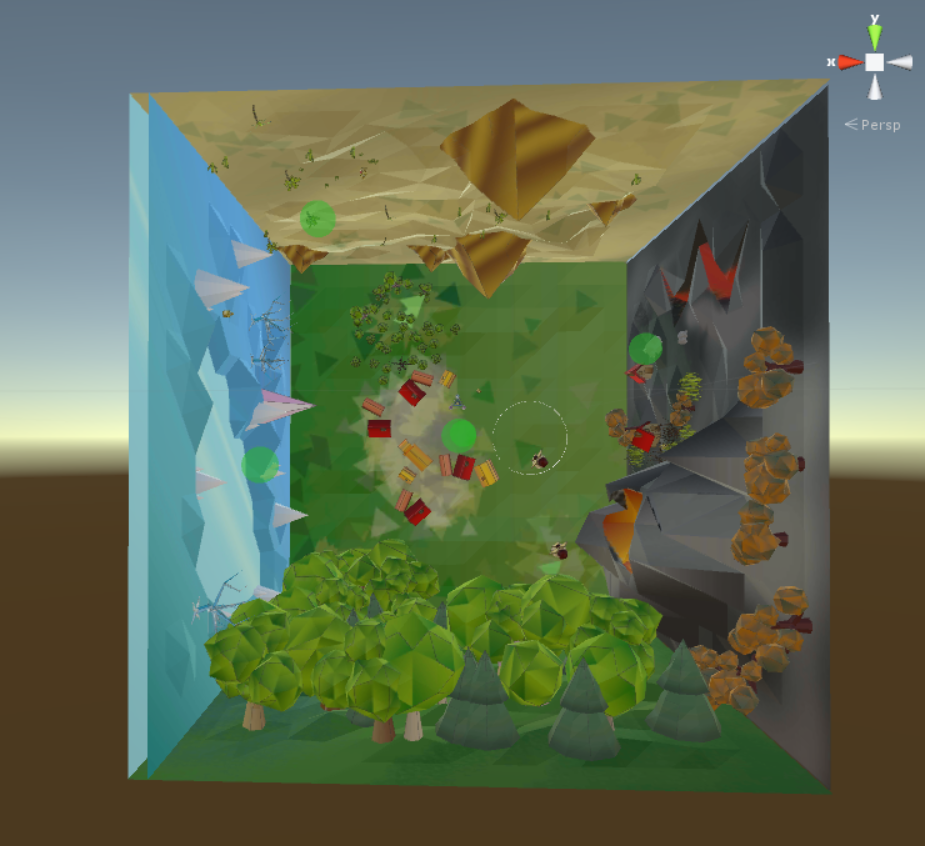
\includegraphics[width=1.0\textwidth]{images/worlds}
	\caption{Einblick in den Weltenwürfel aus Sicht der Gebirgswelt}
	\label{fig:Worlds}
\end{figure}

Das Spiel beziehungsweise der Würfel und seine Innenseiten bestehen aus insgesamt sechs Welten. Anstelle eines einzigen Themas für den gesamten Würfel, gibt es mehrere Themen innerhalb des Würfels geben, da unterschiedliche Themen mehr Potenzial für die Aufgabengenerierung bieten. Die Themen sollen nach ihrer Gegensätzlichkeit zueinander ausgewählt werden und dabei gleichzeitig in Bezug zu den vier Elementen des Seins stehen: Feuer, Wasser, Erde und Luft. Dadurch sind die Themen auch kontextuell miteinander verbunden. Die Welten, die sich im Würfel gegenüber liegen, bilden ein Paar, welchem ein gegensätzliches Thema zu Grunde liegen soll. Pro Paar ist der Spieler dazu aufgefordert, eine Aufgabe zu bewältigen, welche in Abhängigkeit zu den Paarwelten steht. Für die Aufgaben gibt es in jeder Welt eine aktive Zone, in welcher sich Triggerpunkte sowie Viewpoints befinden und mit denen der Nutzer interagieren soll.

Es werden folgende Themen für die Welten im Leveldesign umgesetzt: 

Gebirge und Dorf: Spiegeln die Elemente Luft und Erde wieder. 
Feuer und Eis: Stehen für die Elemente Feuer und Wasser.
Wüste und Wald: Repräsentieren die Elemente Feuer und Erde.